\begin{figure*}[!t]
\centerline{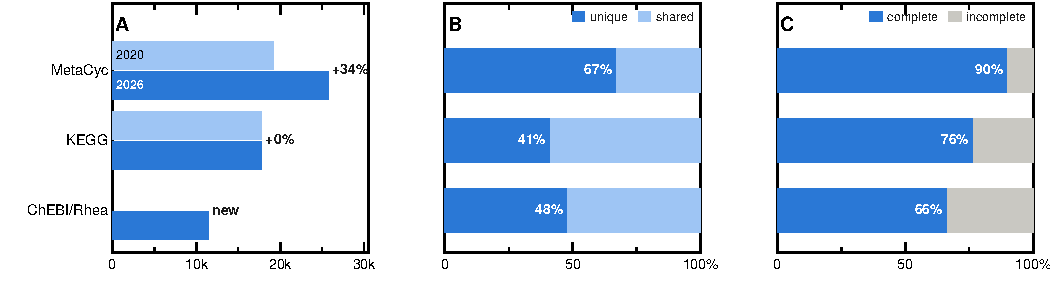
\includegraphics[width=0.88\textwidth,page=1]{figures/main_figures_draft.pdf}}
\caption{\textbf{Structure sources.} (\textbf{A}) Compounds contributed by each
structure-supplying source, 2020 against 2026. KEGG is static; growth is
MetaCyc and the newly-integrated ChEBI. (\textbf{B}) How far each source's
structures reach into the database. Sources overlap, so the bars do not sum to
the 36,943 compounds carrying a structure.}
\label{fig:growth}
\end{figure*}

%% Table 1 is the only table in the main text; the per-source breakdown that was
%% Table 3 in 2020 moves to Supplementary Table S1.
\subsection{Growth and structure coverage}\label{sec:results-growth}

The database has grown 34\% in compounds and 55\% in reactions since 2020
(Table~\ref{tab:growth}), driven mainly by MetaCyc and the BioCyc family.
Structure coverage rose from 28,120 to 36,943 compounds in absolute terms while
slipping from 83\% to 81\% as a rate, because compounds are ingested faster
than structures can be curated for them.

Only three sources supply structures that reach ModelSEED compounds
(Figure~\ref{fig:growth}). MetaCyc reaches 18,801, KEGG 15,278 and ChEBI 9,446
of the 36,943 structured compounds; the sets overlap heavily, and Rhea, despite
contributing 17,477 reactions, supplies structures for none. KEGG is
essentially static --- 17,760 to 17,803 compounds in six years --- so
structural growth is almost entirely MetaCyc and the newly-integrated ChEBI.

\begin{table}[!t]
\caption{Growth since the 2020 release. Per-source counts are in
Supplementary Table~S1.}\label{tab:growth}
\begin{tabular}{lrrr}
\toprule
& 2020 & 2026 & change \\
\midrule
Compounds            & 33,992 & 45,708 & +34\% \\
\quad with structure & 28,120 & 36,943 & +31\% \\
Reactions            & 36,193 & 56,012 & +55\% \\
\quad mass-balanced  & 25,457 & 34,370 & +35\% \\
\botrule
\end{tabular}
\end{table}
